\documentclass{beamer}
\usepackage{amsmath}
\usepackage[english]{babel} %set language; note: after changing this, you need to delete all auxiliary files to recompile
\usepackage[utf8]{inputenc} %define file encoding; latin1 is the other often used option
\usepackage{csquotes} % provides context sensitive quotation facilities
\usepackage{graphicx} %allows for inserting figures
\usepackage{booktabs} % for table formatting without vertical lines
\usepackage{textcomp} % allow for example using the Euro sign with \texteuro
\usepackage{stackengine}
\usepackage{wasysym}
\usepackage{tikzsymbols}
\usepackage{textcomp}
% ELIMINAR COMANDOS DE NAVEGACION%%%%%%%%%%%
\setbeamertemplate{navigation symbols}

%\newcommand{\bubblethis}[2]{
 %       \tikz[remember picture,baseline]{\node[anchor=base,inner sep=0,outer sep=0]%
 %       (#1) {\underline{#1}};\node[overlay,cloud callout,callout relative pointer={(0.2cm,-0.7cm)},%
 %       aspect=2.5,fill=yellow!90] at ($(#1.north)+(-0.5cm,1.6cm)$) {#2};}%
 %   }%
%\tikzset{face/.style={shape=circle,minimum size=4ex,shading=radial,outer sep=0pt,
 %       inner color=white!50!yellow,outer color= yellow!70!orange}}

%% Some commands to make the code easier
\newcommand{\emoticon}[1][]{%
  \node[face,#1] (emoticon) {};
  %% The eyes are fixed.
  \draw[fill=white] (-1ex,0ex) ..controls (-0.5ex,0.2ex)and(0.5ex,0.2ex)..
        (1ex,0.0ex) ..controls ( 1.5ex,1.5ex)and( 0.2ex,1.7ex)..
        (0ex,0.4ex) ..controls (-0.2ex,1.7ex)and(-1.5ex,1.5ex)..
        (-1ex,0ex)--cycle;}
\newcommand{\pupils}{
  %% standard pupils
  \fill[shift={(0.5ex,0.5ex)},rotate=80] 
       (0,0) ellipse (0.3ex and 0.15ex);
  \fill[shift={(-0.5ex,0.5ex)},rotate=100] 
       (0,0) ellipse (0.3ex and 0.15ex);}

\newcommand{\emoticonname}[1]{
  \node[below=1ex of emoticon,font=\footnotesize,
        minimum width=4cm]{#1};}
\usepackage{scalerel}
\usetikzlibrary{positioning}
\usepackage{xcolor,amssymb}
\newcommand\dangersignb[1][2ex]{%
  \scaleto{\stackengine{0.3pt}{\scalebox{1.1}[.9]{%
  \color{red}$\blacktriangle$}}{\tiny\bfseries !}{O}{c}{F}{F}{L}}{#1}%
}
\newcommand\dangersignw[1][2ex]{%
  \scaleto{\stackengine{0.3pt}{\scalebox{1.1}[.9]{%
  \color{red}$\blacktriangle$}}{\color{white}\tiny\bfseries !}{O}{c}{F}{F}{L}}{#1}%
}
\usepackage{fontawesome} % Social Icons
\usepackage{epstopdf} % allow embedding eps-figures
\usepackage{amsmath,amssymb,amsthm} %advanced math facilities
\usepackage{lmodern} %uses font that support italic and bold at the same time

\usepackage{tikz}
\usetikzlibrary{shapes,arrows.meta,positioning}

\usepackage{tcolorbox}

\usefonttheme[onlymath]{serif} %set math font to serif ones

\definecolor{beamerblue}{rgb}{0.2,0.2,0.7} %define beamerblue color for later use

%%% defines highlight command to set text blue
\newcommand{\highlight}[1]{{\color{blue}{#1}}}


%%%%%%% commands defining backup slides so that frame numbering is correct

\newcommand{\backupbegin}{
   \newcounter{framenumberappendix}
   \setcounter{framenumberappendix}{\value{framenumber}}
}
\newcommand{\backupend}{
   \addtocounter{framenumberappendix}{-\value{framenumber}}
   \addtocounter{framenumber}{\value{framenumberappendix}}
}

%%%% end of defining backup slides

%Specify figure caption, see also http://tex.stackexchange.com/questions/155738/caption-package-not-working-with-beamer
\setbeamertemplate{caption}{\insertcaption} %redefines caption to remove label "Figure".
%\setbeamerfont{caption}{size=\scriptsize,shape=\itshape,series=\bfseries} %sets figure  caption bold and italic and makes it smaller


\usetheme{Boadilla}

\usepackage{hyperref}

\newtcolorbox{boxA}{
    fontupper = \bf,
    boxrule = 1.5pt,
    colframe = black % frame color
}
% --------------------
% Overall information
% --------------------
\title[Economía I]{Economía I \vspace{4mm}
\\ Magistral 9: Teoría de Juegos}
\date{}
\author[Riottini]{Franco Riottini}
\vspace{0.4cm}
\institute[]{Universidad de San Andrés} 

\begin{document}

\begin{frame}
\titlepage
\centering

\includegraphics[scale=0.2]{../Figures/logoUDESA.jpg} 
\end{frame}

% \begin{frame}
%     \begin{boxA}
%         \centering
%         CAMBIOS EN EL CRONOGRAMA DE LECTURAS!
%     \end{boxA}
% \end{frame}

\begin{frame}{Dilemas Sociales}
    \begin{itemize}
        \item La interacción estratégica puede generar ciertos desvíos
        \item Cuando hay una interacción estratégica, el resultado de un agente depende no solo de lo que hace ese agente, sino también en gran medida, de cómo actúan o reaccionan otros agentes
        \item Una parte de la economía estudia este tipo de dilemas sociales
        \item Para modelar estos dilemas sociales y distintos tipos de interacciones sociales se suele utilizar lo que se conoce como teoría de juegos
    \end{itemize}
\end{frame}

\begin{frame}{Teoría de juegos}
    \begin{itemize}
        \item Estudia de manera formal y abstracta las decisiones óptimas que deben tomar diversos adversarios en conflicto
        \item Es el estudio matemático de la toma de decisiones, del conflicto y la estrategia en situaciones sociales
        \item Jugadores que toman decisiones que se consideran estratégicas
        \begin{itemize}
            \item los jugadores son entes racionales (no necesariamente humanos)
            \item los entes que participan en el juego actúan teniendo en cuenta las acciones que tomarían los demás
        \end{itemize}
    \end{itemize}
\end{frame}


\begin{frame}{Estudiando juegos}
    \begin{itemize}
        \item El término ``juegos'' refiere básicamente a modelos de interacción estratégica
        \item Es decir, modelos donde las personas involucradas en una interacción social saben que sus acciones afectan a otros y viceversa
        \begin{boxA}
            \centering
            Un juego es cualquier situación en la que los participantes, a los que llamaremos jugadores, toman decisiones estratégicas, es decir, toman en cuenta las acciones y respuestas de los demás.
        \end{boxA}
        \item Estas decisiones estratégicas dan como resultado premios o castigos para
        los jugadores.        
        \item ¿Cómo analizamos interacciones sociales?
        \begin{itemize}
            \item Definimos las características de un juego
            \item Principalmente reglas y resultados
            \item Obtenemos ‘modos de jugar’: analizamos cuales son las decisiones óptimas para los jugadores
        \end{itemize}
    \end{itemize}
\end{frame}

\begin{frame}
    \frametitle{Tipos de juegos}
    \begin{itemize}
        \item Juegos simultáneos: donde se toma una decisión one-shot. Cada agente tuvo que tomar su decisión sin haber observado las del resto.
        \item Juegos secuenciales: donde los jugadores toman sus decisiones de forma consecutiva. Los jugadores tienen alguna información acerca de las elecciones de otros jugadores
    \end{itemize}
\end{frame}

\begin{frame}
    \frametitle{Elementos de un juego}
    \begin{itemize}
        \item \textbf{Los jugadores:} Quién está interactuando con quién.
        \item \textbf{Las estrategias viables:} Qué acciones están abiertas a los jugadores.
        \item \textbf{La información:} Lo que cada jugador sabe al tomar su decisión.
        \begin{itemize}
            \item Información perfecta: todos los jugadores conocen los movimientos realizados previamente por el resto de jugadores (solo en juegos secuenciales).
            \item Información completa: cada jugador conoce las estrategias y recompensas del resto de jugadores, pero no tiene porqué conocer las acciones de estos.
        \end{itemize}
        \item \textbf{Los pagos:} Cuáles serán los resultados para cada una de las posibles combinaciones de acciones.\vspace{4mm}
    \end{itemize}
\end{frame}

\begin{frame}{Juegos Simultaneos}
    \begin{itemize}
        \item Los jugadores deciden a la vez o bien desconocen los movimientos anteriores de los otros jugadores.
        \item Tenemos dos productores: Jorge y Walter.
        \item Cada uno debe decidir cuanto producir tomando en cuenta lo que piensa que hará el otro.
        \item Estrategias:
        \begin{itemize}
            \item Walter está analizando colocar una plantación de manzanas o plantar trigo.
            \item Jorge está analizando si iniciar una producción de miel o plantar trigo.
        \end{itemize}
        \item Para resolver el juego es util construir una \textbf{matriz de pagos}

        \centering
        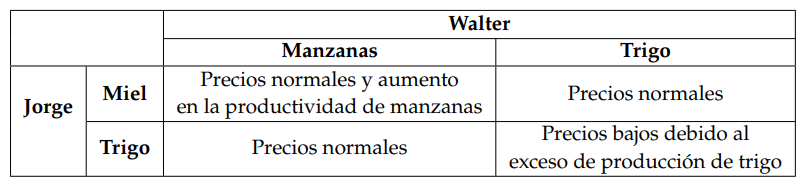
\includegraphics[scale=0.6]{../Figures/T20.1.png}

    \end{itemize}
\end{frame}

\begin{frame}{Representación Normal del juego}
    \centering
    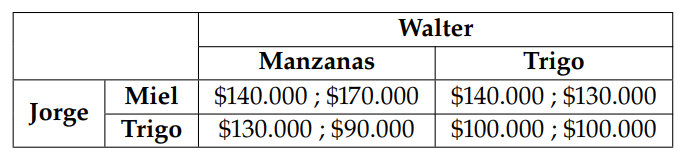
\includegraphics[scale=0.6]{../Figures/T20.2.png}
    \begin{boxA}
        \centering
        Esta matriz se denomina representación normal de un juego. Un
juego está representado en forma normal cuando la lista de todos
los posibles resultados de cada jugador, con todas las posibles
combinaciones de estrategias, viene dada para cualquier secuencia
de decisiones en el juego.
    \end{boxA}
\end{frame}

\begin{frame}{Resolviendo el juego}
    
    \begin{itemize}
        \item Es útil pensar que cada uno quiere tomar la mejor decisión posible\dots
        \item ¿Cuál es la mejor respuesta de cada individuo?
        \item La mejor respuesta es aquella estrategia que le da al jugador el mayor pago, dada la estrategia que elige el otro jugador.
        \begin{boxA}
            \centering
            Se denomina mejor respuesta a aquella estrategia que proporciona al jugador el pago más elevado, condicional a lo que se conjetura que harán los demás.
        \end{boxA}
    \end{itemize}
\end{frame}

\begin{frame}{Mejor respuesta de Jorge}
    
    Si independientemente de lo que elige Walter, a Jorge siempre le conviene hacer lo mismo, decimos que producir miel es una \textbf{estrategia dominante} para Jorge.
    
    \centering
    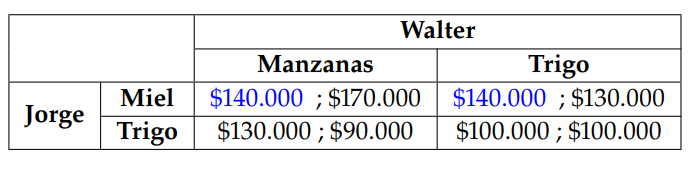
\includegraphics[scale=0.6]{../Figures/T20.3.png}

    \begin{boxA}
        \centering
        Una estrategia dominante es una mejor respuesta a todas las posibles estrategias de otro jugador. Si un agente tiene una estrategia dominante siempre la va a jugar, independientemente de la estrategia que juegue el rival.
    \end{boxA}
\end{frame}

\begin{frame}{Mejor respuesta de Walter}
    \centering
    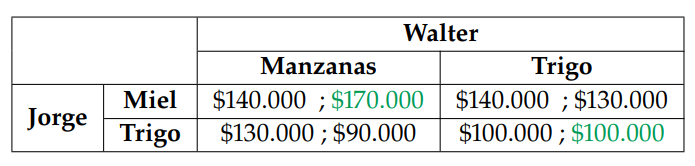
\includegraphics[scale=0.6]{../Figures/T20.4.png}
\end{frame}

\begin{frame}{Equilibrio de Nash}
    Un perfil de estrategias es un equilibrio de Nash si, dadas las estrategias del rival, cada uno de los agentes está jugando su mejor respuesta.
    \begin{boxA}
        \centering
        En un equilibrio de Nash, ninguno de los jugadores tiene incentivos a desviarse, debido a que no puede obtener un pago mayor cambiando de estrategia.
    \end{boxA}
    \centering
    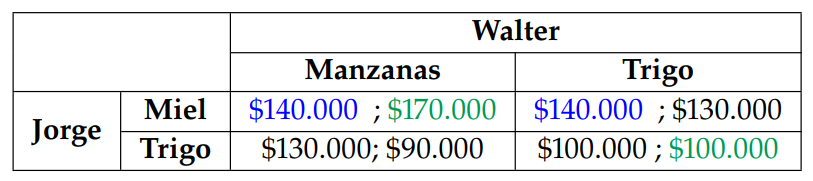
\includegraphics[scale=0.6]{../Figures/T20.5.png}
\end{frame}

\begin{frame}{Equilibrio Pareto Eficiente}
    \begin{center}
        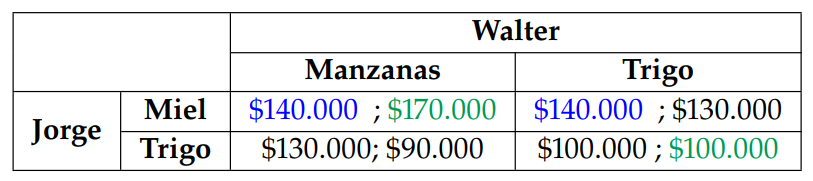
\includegraphics[scale=0.6]{../Figures/T20.5.png}
    \end{center}
    Este resultado también permite que Walter y Jorge obtengan el mejor resultado posible. Si esto sucede, decimos que se alcanza un resultado \textbf{Pareto eficiente}.
    \begin{boxA}
        \centering
        En un equilibrio Pareto eficiente, no hay otra situación o alternativa en donde uno esté mejor y ninguno esté peor. 
    \end{boxA}
    Este es el concepto de eficiencia del que hablamos al principio de la materia, donde decíamos que una asignación era \textbf{eficiente} si no podíamos mejorar la situación de un agente sin empeorar la de otro.
\end{frame}

\begin{frame}{Equilibrios Multiples}
    Existen situaciones en las que un juego puede tener más de un equilibrio de Nash.
    \begin{itemize}
        \item Agus y Juani son dos hermanos que quieren ir al cine a ver una película.
        \item Juani prefiere ver el drama y Agus prefiere la película de acción. 
        \item Ambos valoran más el hecho de ir juntos a ver su película favorita solos.
    \end{itemize}
    \begin{center}
        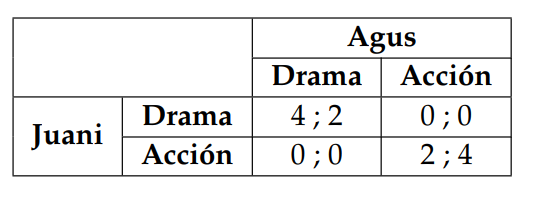
\includegraphics[scale=0.5]{../Figures/T20.6.png}
        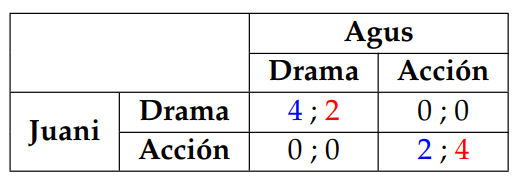
\includegraphics[scale=0.5]{../Figures/T20.7.png}
    \end{center}
\end{frame}

\begin{frame}{El dilema del prisionero}
    \begin{itemize}
        \item Dos potenciales criminales son arrestados y se les ofrece un trato.
        \begin{itemize}
            \item Si ninguno confiesa, ambos serán sentenciados a un mes de cárcel.
            \item Si ambos confiesan, serán sentenciados a seis meses de cárcel.
            \item Si uno confiesa y el otro no, el que confesó será puesto inmediatamente en libertad, mientras que el que no confesó será condenado a nueve meses (seis por el robo y tres por obstrucción a la justicia).
        \end{itemize}
        \item Cada jugador cuenta con dos posibles estrategias: confesar o no confesar
    \end{itemize}
    \begin{center}
        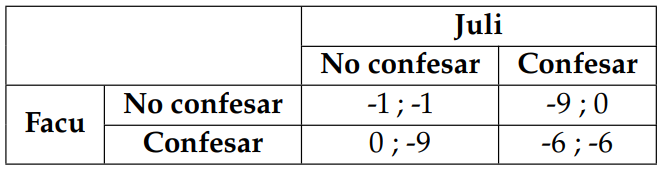
\includegraphics[scale=0.6]{../Figures/T20.8.png}
    \end{center}
\end{frame}
\begin{frame}{El dilema del prisionero}
    \begin{center}
        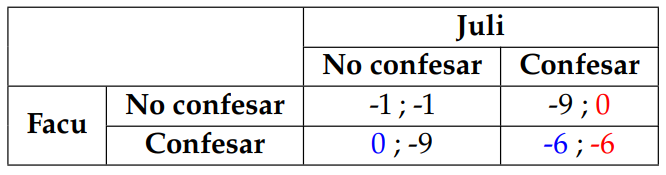
\includegraphics[scale=0.6]{../Figures/T20.9.png}
    \end{center}
    \begin{itemize}
        \item El equilibrio de Nash es que ambos confiesen.
        \item Tampoco querran cambiar su decisión luego de ver el resultado.
        \item Se genera un dilema desde el punto de vista cooperativo.
        \item Este resultado es subóptimo.
        \item Se trata de un \textbf{equilibrio en estrategias dominantes}: siempre van a elegir confesar, no importa lo que juegue el rival.
    \end{itemize}
    \begin{boxA}
        \centering
        El principal impedimento para que los jugadores lleguen a este equilibrio superador es que siempre existirán incentivos para desviarse de cualquier par de estrategias que no sean el equilibrio de Nash
    \end{boxA}
\end{frame}

\begin{frame}{¿Como se sale del dilema?}
    \begin{itemize}
        \item ¿Cómo podemos llegar al resultado de cooperación?
        \item Juegos repetidos:
        \begin{itemize}
            \item Los jugadores pueden establecer castigos en base a lo actuado en las diferentes instancias del juego.
            \item  Si uno se desvía del comportamiento que piensa que corresponde, el otro lo castigará en los próximos períodos.
        \end{itemize}
        \item Incorporar dilemas morales
        \begin{itemize}
            \item Juego del ultimátum.
            \item No delatar es "lo que está bien"
        \end{itemize}
    \end{itemize}
\end{frame}


\begin{frame}{Juegos Secuenciales}
    \begin{itemize}
        \item Los jugadores toman decisiones en forma consecutiva, es decir, primero decide un jugador y luego el otro.
        \item Ya no podemos presentar el juego en forma de cuadro, sino que tenemos lo que se denomina \textbf{representación en forma extensiva} de un juego.
        \item Para resolvernos ya no nos va a alcanzar encontrar la mejor respuesta, sino que vamos a tener que utilizar \textbf{inducción hacia atrás}.
    \end{itemize}
\end{frame}

\begin{frame}{El robo al Banco Rio}
    \begin{itemize}
        \item Dos ladrones entran a un reconocido banco.
        \item Se llevan \$200 millones pero al escapar se los lleva el ladron 1, prometiendo que le enviará la mitad al ladron 2.
        \item El ladron 2 decide amenazarlo, con que si no cumple la promesa lo denunciará a la policía
        \item El ladron 1 decide primero... cumplir la promesa o no cumplirla y enviarle solo \$25 millones 
        \item El Ladrón 2 va a decidir segundo, luego de observar qué hizo el Ladrón 1. Sus estrategias van a ser: tomar lo que el Ladrón 1 le envió o denunciarlo a la policía.
    \end{itemize}
\end{frame}

\begin{frame}{El robo al Banco Rio}
    \begin{center}
        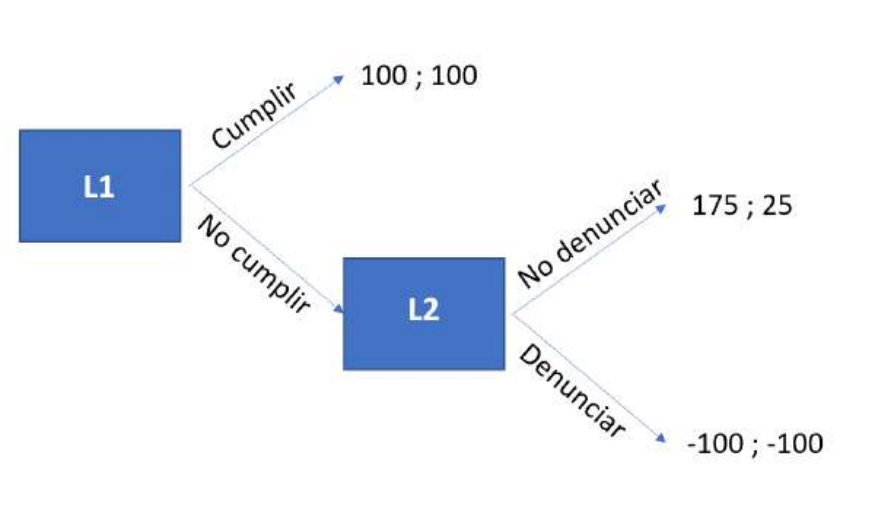
\includegraphics[scale=0.6]{../Figures/C20.2.png}
    \end{center}
\end{frame}


\begin{frame}{El robo al Banco Rio}
    \begin{itemize}
        \item Para resolver este problema, vamos a utilizar la inducción hacia atrás.
        \item Lo primero que vamos a hacer es observar qué le conviene hacer al Ladrón 2 si el Ladrón 1 no cumple su promesa.
        \item Si el Ladrón 1 no cumple su promesa, al Ladrón 2 ¿le conviene aceptar o no aceptar? Como su pago es \$25 millones si acepta y -\$100 millones si no acepta, claramente
        le convendrá aceptar.
        \item Si el Ladrón 2 amenaza con denunciar al Ladrón 1, decimos que nos encontramos ante una "amenaza no creíble".
        \item El Ladrón 2 no tendrá incentivos para cumplir con su palabra.
        \begin{boxA}
            \centering
            Con la inducción hacia atras, recorremos ``hacia atrás'' el ``arbol'' hasta llegar
            al nodo inicial, identificando en cada nodo la estrategia óptima en
            anticipación del comportamiento que se espera hacia adelante.            
        \end{boxA}
    \end{itemize}
\end{frame}

\begin{frame}{Conclusión}
    \begin{itemize}
        \item No todo es color de rosas como cuando veíamos comercio.
        \item Ciertos comportamientos y ciertas configuraciones pueden generar resultados que no sean los óptimos desde el punto de vista social.
        \item Existen otras configuraciones, como los juegos con \textbf{estrategias mixtas} donde ya no tenemos certeza, sino que asignamos probabilidades a las estrategias de los jugadores.
        \item La teoría de juegos es una herramienta muy útil para entender y modelar comportamientos estratégicos.
        \item Además, es util para pensar en los efectos de políticas públicas y en las expectativas que tienen los agentes.
    \end{itemize}
\end{frame}

\end{document}